% Supplementary material for the PSS technical report.
% Compile with pdflatex (no bibliography needed).

\documentclass[10pt]{article}

\usepackage[T1]{fontenc}
\usepackage[utf8]{inputenc}
\usepackage{times}
\usepackage[margin=0.85in]{geometry}
\usepackage{graphicx}
\usepackage{booktabs}
\usepackage{caption}
\usepackage{hyperref}
\newcommand{\pss}{PSS}

\title{Supplementary Material for\\\pss: A Cognitive Runtime Above Perception}
\author{Jiahe Qi\\Independent Researcher}
\date{November 2026}

\begin{document}
\setlength{\tabcolsep}{8pt}
\renewcommand{\arraystretch}{1.05}

\maketitle

\section{Additional Diagnostics}

\begin{figure}[ht]
\centering
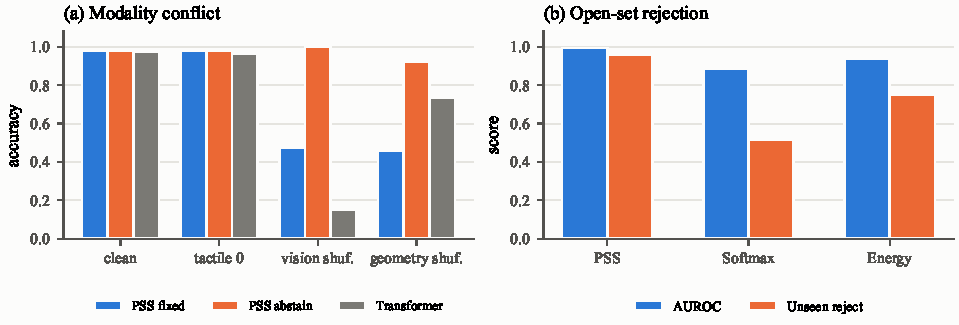
\includegraphics[width=\linewidth]{figures/fig_conflict_openset.pdf}
\caption{(a) Modality conflict: \pss fixed fusion vs abstention vs the
transformer. Under a shuffled vision channel, abstention keeps accepted accuracy
at 1.000 with coverage 0.083; the transformer has no explicit abstention.
(b) Open-set AUROC and unseen rejection.}
\label{fig:conflict-openset}
\end{figure}

\begin{figure}[ht]
\centering
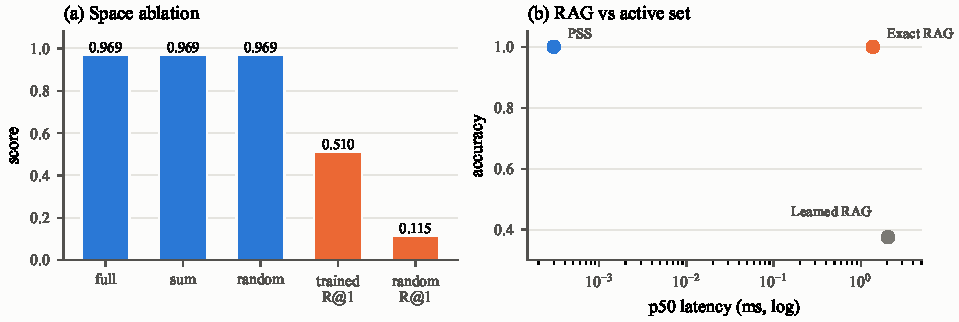
\includegraphics[width=\linewidth]{figures/fig_space_rag.pdf}
\caption{(a) Closed-set accuracy is invariant across the full, summed, and
random-projection spaces; the learned projection's value is cross-modal R@1
(0.510 vs 0.115). (b) Exact RAG matches accuracy but scans the full history;
the \pss active set is a constant-time lookup.}
\label{fig:space-rag}
\end{figure}

\begin{figure}[ht]
\centering
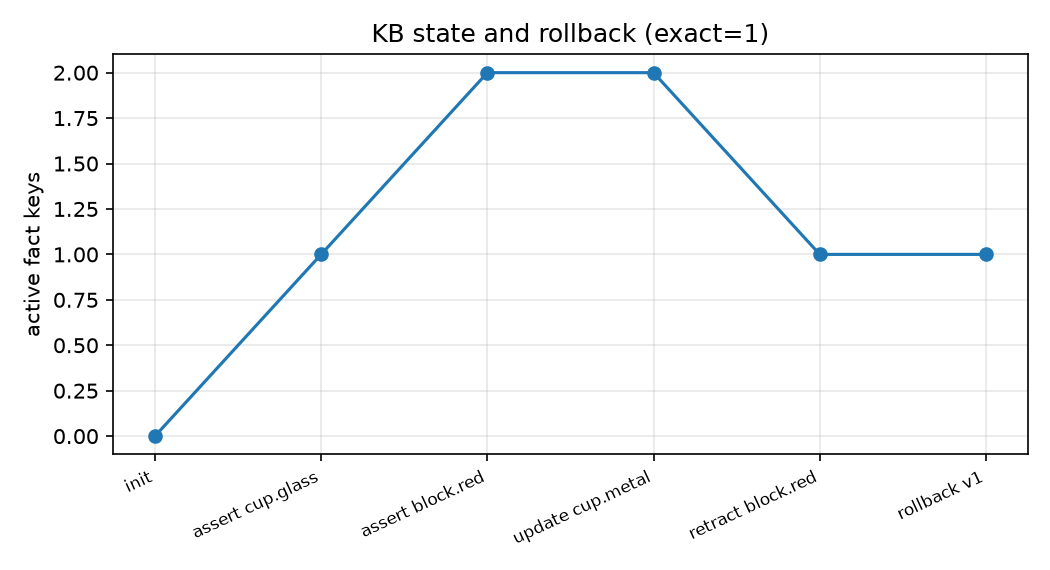
\includegraphics[width=0.85\linewidth]{figures/fig2_kb_state.png}
\caption{Knowledge-base state and rollback. A rollback restores the business
state hash exactly; the audit log records the change.}
\label{fig:kb}
\end{figure}

The additional diagnostics support the discussion rather than a separate claim.
The conflict result shows that abstention can preserve accepted accuracy at low
coverage. The space ablation shows that the learned projection's value is
alignment, not closed-set accuracy. The RAG result shows that the active-set
advantage is a cost advantage against a strong retriever.

\section{Additional Figures}

\begin{figure}[ht]
\centering
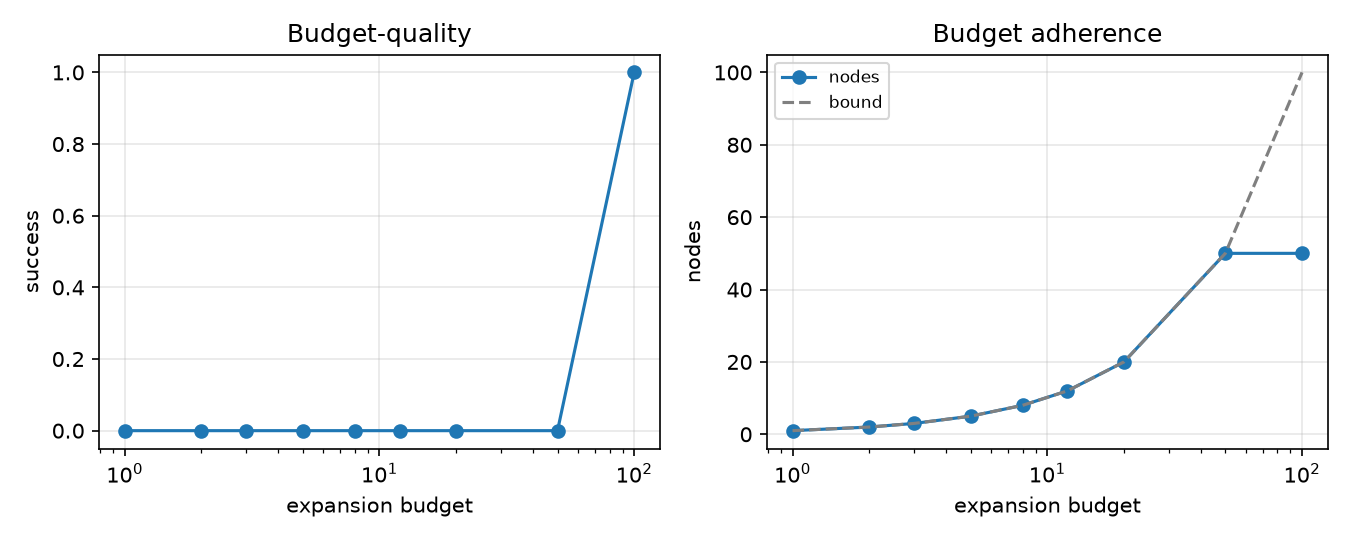
\includegraphics[width=0.85\linewidth]{figures/fig3_budget_quality.png}
\caption{Quality versus budget. The planner is anytime: quality is monotone in
the budget, and the budget controller keeps the node count within the cap.}
\label{fig:budget}
\end{figure}

\section{Additional Tables}

\begin{table}[ht]
\centering
\small
\begin{tabular}{@{}lcc@{}}
\toprule
Relation type & F1 (clean) & F1 (tactile removed) \\
\midrule
spatial & 0.957 & -- \\
semantic & 0.996 & -- \\
tactile & 0.970 & 0.483 \\
\bottomrule
\end{tabular}
\caption{Typed relation heads. Removing tactile drops tactile F1 to 0.483,
which shows the head is not using a shortcut.}
\label{tab:relations}
\end{table}

\begin{table}[ht]
\centering
\small
\begin{tabular}{@{}p{0.44\linewidth}p{0.46\linewidth}@{}}
\toprule
Setting & Result \\
\midrule
re-ID candidates, $k=1$ + fallback & 0.972 $\rightarrow$ 1.000, $\sim$1.2 candidates \\
compute, $N=200$ / $N=1000$ & 6.4$\times$ / 23.6$\times$ \\
long-history fact, $k=4$: hot / old learned / query-conditioned & 0.237 / 0.241 / 1.000 \\
exact-RAG vs \pss latency & 1.38 ms vs 0.0003 ms \\
\bottomrule
\end{tabular}
\caption{Active-set memory and bounded inference. The long-history negative
result is explained by query-independent scoring; a simple query-recency rule
matches the learned policy.}
\label{tab:memory}
\end{table}

\begin{table}[ht]
\centering
\small
\begin{tabular}{@{}lccc@{}}
\toprule
Expert family & Vision zero-shot & Tactile zero-shot & Vision $k=1$ \\
\midrule
\texttt{category\_pretrain} & 0.200 & 0.067 & 1.000 \\
\texttt{category\_pretrain\_instance} & 0.167 & 0.067 & 0.900 \\
\texttt{category\_pretrain\_instance8} & 0.192 & 0.100 & 0.908 \\
\bottomrule
\end{tabular}
\caption{Cross-family swap and one-shot calibration (chance 0.167). The public
space is a calibratable interface, not a zero-shot coordinate system.}
\label{tab:families}
\end{table}

\begin{table}[ht]
\centering
\small
\begin{tabular}{@{}lcc@{}}
\toprule
Variant & ID retention & Switches \\
\midrule
full & 1.000 & 0.00 \\
\texttt{no\_memory} & 0.827 & 0.56 \\
\texttt{no\_entity} & 0.270 & 47.47 \\
\bottomrule
\end{tabular}
\caption{L2 bundle replay on the same detection stream (valid 19/33 bundles).
The state-layer ablation, not perception, explains the difference.}
\label{tab:l2-bundles}
\end{table}

\section{Claim--Evidence Map}

\begin{table}[ht]
\centering
\small
\begin{tabular}{@{}p{0.18\linewidth}p{0.46\linewidth}p{0.20\linewidth}@{}}
\toprule
Claim & Evidence & Strength \\
\midrule
C1 state & audit 1.00; 70-frame 0.989 vs 0.500; L2 1.000/0.827/0.270 & medium--strong \\
C2 relations & F1 0.957/0.996/0.970; hybrid 0.857 vs 0.828 & medium \\
C3 memory & 1.2 candidates; 6.4$\times$/23.6$\times$; query 0.241$\rightarrow$1.000 & medium--strong \\
C4 contracts & SSR/RBE/INT/RCR invariant; contract-free 0/9; scale flat & strong \\
C5 protocol & N1--N8; twins; preregistration; contract-free baseline & strong \\
C6 interface & zero-shot 0.186; $k=1$ 0.936; tactile 0.067--0.100 & medium--strong \\
\bottomrule
\end{tabular}
\caption{Compact claim--evidence map. The full version is in the repository.}
\end{table}

\end{document}
